% !TeX TXS-program:compile = txs:///pythonlualatex

\documentclass[a4paper,11pt]{article}
\usepackage[sujet,pythontex]{cp-base}
\graphicspath{{./graphics/}}
%variables
\donnees[
	classe={1\up{ère} 2M2},matiere={[SPÉ.MATHS]},mois={Jeudi 3 Février},annee=2022,duree=1h30,typedoc=DS,numdoc=5
]
%formatage
\author{Pierquet}
\title{\nomfichier}
\hypersetup{pdfauthor={Pierquet},pdftitle={\nomfichier},allbordercolors=white,pdfborder=0 0 0,pdfstartview=FitH}
%divers
\lhead{\entete{\matiere}}
\chead{\entete{\lycee}}
\rhead{\entete{\classe{} - \mois{} \annee}}
\lfoot{\pied{\matiere}}
\cfoot{\logolycee{}}
\rfoot{\pied{\numeropagetot}}
\fancypagestyle{enteteds}{\fancyhead[L]{\entete{Durée : \duree}}}

\begin{document}

\pagestyle{fancy}

\thispagestyle{enteteds}

\setcounter{numexos}{0}

\part{DS05 - Second degré, probabilités, trigonométrie, \ldots}

\smallskip

\nomprenomtcbox

\begin{marker}$\leftrightsquigarrow$ Le sujet est à rendre avec la copie. $\leftrightsquigarrow$\end{marker}

\exonum{6}

\begin{enumerate}
	\item Déterminer le tableau de signes des expressions suivantes :
	\begin{enumerate}
		\item $2x^2+4x-30$ ;
		\item $\dfrac{2x+6}{x^2-3x+2}$.
	\end{enumerate}
	\item Résoudre les inéquations suivantes :
	\begin{enumerate}
		\item $(10-x)(x^2-6x+9)<0$ ;
		\item $\dfrac{2x+6}{x^2-3x+2} \pg 0$.
	\end{enumerate}
\end{enumerate}

\medskip

\exonum{5}

\medskip

En vue de sa prochaine brochure d'information sur les dangers des Réseaux Sociaux, un lycée a fait remplir un questionnaire à chacun des \num{2000}~élèves, répartis dans les sections de seconde, première et terminale. On obtient la répartition : 

\begin{itemize}
	\item un quart des élèves est en terminale ; 
	\item 35\,\% des élèves sont en première ; 
	\item tous les autres sont en seconde ; 
	\item parmi les élèves de terminale, 70\,\% utilisent régulièrement les Réseaux Sociaux ; 
	\item 630 élèves sont des élèves de première qui utilisent régulièrement les Réseaux Sociaux. 
	\item \num{1740}~élèves utilisent régulièrement les Réseaux Sociaux.
\end{itemize}

Cette enquête permet de modéliser le choix d'un élève du lycée. On choisit au hasard un questionnaire d'élève en supposant que ce choix se fait en situation d'équiprobabilité. On note :

\begin{itemize}
	\item $S$ l'évènement \og le questionnaire est celui d'un élève en classe de seconde \fg ;
	\item $E$ l'évènement \og le questionnaire est celui d'un élève en classe de première \fg ;
	\item $T$ l'évènement \og le questionnaire est celui d'un élève en classe de terminale \fg ;
	\item $R$ l'évènement \og le questionnaire est celui d'un élève qui utilise régulièrement les Réseaux Sociaux (RS) \fg.
\end{itemize}

\begin{enumerate}
	\item Compléter le tableau d'effectifs ci-dessous.
	
	\smallskip
	
	\begin{tblr}{%
			width=\linewidth,colspec={l*{4}{X[c]}},
			vline{1}={2-Z}{solid},vline{2-Z}={solid},hline{1}={2-Z}{solid},hline{2-Z}={solid},
			rows={font=\sffamily}
			}
											& Seconde & Première & Terminale & Total\\
		Utilise régulièrement les RS 		&	&630&	&		\\
		N'utilise pas régulièrement les RS 	&	&	&	&		\\
		Total 								&	&	&	&2\,000	\\
	\end{tblr}
	\item Déterminer la probabilité d'obtenir le questionnaire d'un élève de seconde qui utilise régulièrement les RS. 
	\item Calculer la probabilité de $R$ sachant $T$, notée $p_{T}(R)$, et interpréter ce résultat à l'aide d'une phrase. 
	\item Calculer la probabilité que le questionnaire choisi soit celui d'un élève qui n'utilise pas les RS. 
	\item Le questionnaire est celui d'un élève qui utilise régulièrement les RS.
	
	Montrer que la probabilité que ce soit le questionnaire d'un élève de première est égale à $\frac{21}{58}$.
\end{enumerate}

\newpage

\exonum{7}

\medskip

Un restaurant propose à sa carte deux types de dessert :

\begin{itemize}
	\item un assortiment de macarons, choisi par 50\,\% des clients; 
	\item une part de tarte tatin, choisie par 30\,\% des clients.
\end{itemize}

20\,\% des clients ne prennent pas de dessert et aucun client ne prend plusieurs desserts. Le restaurateur constate :

\begin{itemize}
	\item que parmi les clients ayant pris un assortiment de macarons, 80\,\% prennent un café ; 
	\item que parmi les clients ayant pris une part de tarte tatin, 60\,\% prennent un café; 
	\item que parmi les clients n'ayant pas pris de dessert, 90\,\% prennent un café.
\end{itemize}

On interroge au hasard un client de ce restaurant. On note $p$ la probabilité associée à cette expérience aléatoire. On note :

\begin{itemize}
	\item $M$ l'évènement : \og Le client prend un assortiment de macarons \fg{} ; 
	\item $T$ l'évènement : \og Le client prend une part de tarte tatin \fg{} ; 
	\item $P$ l'évènement : \og Le client ne prend pas de dessert \fg{} ; 
	\item $C$ l'évènement: \og Le client prend un café \fg{} et $\overline{C}$ l'évènement contraire de $C$.
\end{itemize}

\begin{enumerate}
	\item En utilisant les données de l'énoncé, préciser la valeur de $p(T)$ et celle de $p_{T}(C)$, probabilité de l'évènement $C$ sachant que $T$ est réalisé. 
	\item Recopier et compléter l'arbre ci-dessous: 
	
	\begin{center}
		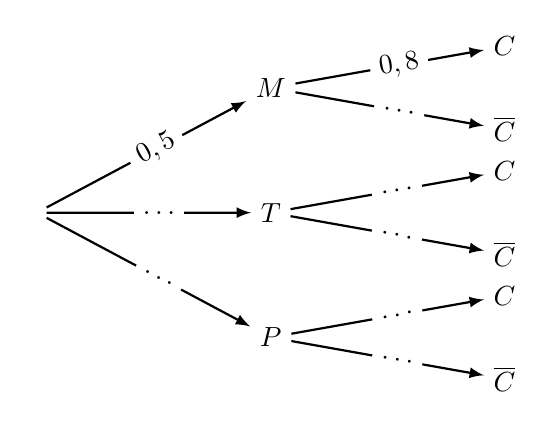
\begin{tikzpicture}[scale=0.66]
			\tikzstyle{fleche}=[->,>=latex,thick]
			\tikzstyle{noeud}=[]
			\tikzstyle{feuille}=[]
			\tikzstyle{etiquette}=[pos=0.55,sloped,fill=white]
			
			\def\DistanceInterNiveaux{3}
			\def\DistanceInterFeuilles{1}
			
			\def\NiveauA{(0)*\DistanceInterNiveaux}
			\def\NiveauB{(1.5)*\DistanceInterNiveaux}
			\def\NiveauC{(3)*\DistanceInterNiveaux}
			\def\InterFeuilles{(-0.8)*\DistanceInterFeuilles}
			
			\node[noeud] (R) at ({\NiveauA},{(4)*\InterFeuilles}) {$ $};
			\node[noeud] (Ra) at ({\NiveauB},{(1)*\InterFeuilles}) {$M$};
			\node[feuille] (Raa) at ({\NiveauC},{(0)*\InterFeuilles}) {$C$};
			%\node[feuille] (Rab) at ({\NiveauC},{(1)*\InterFeuilles}) {$C_{n+1}$};
			\node[feuille] (Rac) at ({\NiveauC},{(2)*\InterFeuilles}) {$\overline{C}$};
			\node[noeud] (Rb) at ({\NiveauB},{(4)*\InterFeuilles}) {$T$};
			\node[feuille] (Rba) at ({\NiveauC},{(3)*\InterFeuilles}) {$C$};
			%\node[feuille] (Rbb) at ({\NiveauC},{(4)*\InterFeuilles}) {$B_{n+1}$};
			\node[feuille] (Rbc) at ({\NiveauC},{(5)*\InterFeuilles}) {$\overline{C}$};
			\node[noeud] (Rc) at ({\NiveauB},{(7)*\InterFeuilles}) {$P$};
			\node[feuille] (Rca) at ({\NiveauC},{(6)*\InterFeuilles}) {$C$};
			%\node[feuille] (Rcb) at ({\NiveauC},{(7)*\InterFeuilles}) {$A_{n+1}$};
			\node[feuille] (Rcc) at ({\NiveauC},{(8)*\InterFeuilles}) {$\overline{C}$};
			
			\draw[fleche] (R)--(Ra) node[etiquette] {$\num{0,5}$};
			\draw[fleche] (Ra)--(Raa) node[etiquette] {$\num{0,8}$};
			\draw[fleche] (Ra)--(Rac) node[etiquette] {$\ldots$};
			\draw[fleche] (R)--(Rb) node[etiquette] {$\ldots$};
			\draw[fleche] (Rb)--(Rba) node[etiquette] {$\ldots$};
			\draw[fleche] (Rb)--(Rbc) node[etiquette] {$\ldots$};
			\draw[fleche] (R)--(Rc) node[etiquette] {$\ldots$};
			\draw[fleche] (Rc)--(Rca) node[etiquette] {$\ldots$};
			\draw[fleche] (Rc)--(Rcc) node[etiquette] {$\ldots$};
		\end{tikzpicture}
	\end{center}
	\item  
	\begin{enumerate}
		\item Exprimer par une phrase ce que représente l'évènement $M \cap C$ puis calculer $p(M \cap C)$. 
		\item Montrer que $p(C) = \num{0,76}$.
	\end{enumerate} 
	\item Quelle est la probabilité que le client prenne un assortiment de macarons sachant qu'il prend un café ?
	\item Les évènements M et C sont-ils indépendants ? Justifier la réponse.
	\item On interroge au hasard, et de manière indépendante, trois clients du restaurant.
	
	Déterminer la probabilité que les trois clients aient pris du café.
\end{enumerate}

\medskip

\exonum{1}

\medskip

Compléter l'agorithme suivant, en \calgpython, afin qu'il \textit{calcule} et \textit{affiche} la probabilité de l'évènement $A \cup B$ :

\begin{envpython}[14cm]
pA = float(input("Saisir la probabilité de A : "))
pB = float(input("Saisir la probabilité de B : "))
pAetB = float(input("Saisir la probabilité de A inter B : "))

pAouB = ........................

print(f"La probabilité de A ou B vaut donc {......}")
\end{envpython}

\newpage

\exonum{6}

\begin{enumerate}
	\item Déterminer la mesure principale, ainsi que le cosinus et le sinus des angles (en radians) suivants :
	\begin{enumerate}
		\item $\dfrac{19\pi}{4}$ ;
		\item $\dfrac{-56\pi}{3}$ ;
		\item $-37\pi$ ;
		\item $\dfrac{99\pi}{6}$.
	\end{enumerate}
	\item Résoudre les équations suivantes :
	\begin{enumerate}
		\item $\cos(x)=-\dfrac{1}{2}$ ;
		\item $\sin(x)=\dfrac{\sqrt{2}}{2}$ ;
		\item $(x+3)(2\cos(x)+2)=0$.
	\end{enumerate}
\end{enumerate}

\medskip

\exonum{5}

\medskip

On considère la fonction $f$ définie sur $\intervFF{0}{3,5}$ par $f(x)=3x^3-16x^2+23x-8$.

\begin{enumerate}
	\item À l'aide de la calculatrice, et du réglage \og automatique \fg{}, tracer \uline{soigneusement} la courbe $\mathscr{C}_f$ représentative de $f$ dans le repère orthogonal suivant, pour lequel l'unité verticale est à préciser.
	%
	\begin{center}
		\begin{tikzpicture}[x=4cm,y=0.8cm,xmin=0,xmax=3.5,xgrille=0.25,xgrilles=0.25,ymin=-8,ymax=6,ygrille=1,ygrilles=0.25]
		\tgrilles \tgrillep \axestikz*
		\axextikz[font=\sffamily]{0.25,0.5,...,3.25} \axeytikz*{-8,-7,...,5}
		%\draw[very thick,red,domain=0:3.5,samples=250] plot (\x,{3*\x*\x*\x-16*\x*\x+23*\x-8}) ;
	\end{tikzpicture}
	\end{center}
	\item Graphiquement :
	\begin{enumerate}
		\item résoudre l'équation $f(x)=0$ ;
		\item déterminer le tableau de signes de $f(x)$ ;
		\item déterminer le tableau de variations de $f$.
	\end{enumerate}
	\item[Bonus] En utilisant les \og outils graphiques \fg{} de la calculatrice, déterminer une équation de la tangente à $\mathscr{C}_f$ au point d'abscisse $2$.
\end{enumerate}

\end{document}